
Detalhes do barramento e processo de concepção.

\section{O que é HBUS e o seu objetivo}

O barramento HBUS é uma especificação desenvolvida para explorar possibilidades de automação doméstica, daí seu nome, derivado de \textit{Home Bus}.

A especificação contém definições tanto de hardware e software para acomodar a troca de informações entre os dispositivos que participam de uma rede de automação doméstica.

Além de ser uma ferramenta desenvolvida para a exploração e aquisição de conhecimento na área de automação, o conjunto de soluções aplicadas mostrou-se muito capaz de funcionar de forma coerente.

\section{O processo de concepção inicial}

Antes de mais nada, é necessário pensar um pouco para que o projeto tenha sentido e seja realizável.

\subsection{A filosofia de alocação de recursos}

Todo o projeto foi pensado de forma a ser flexível e as especificações podem ser atendidas por uma gama enorme de plataformas e meios físicos de transporte de dados.

No entanto, as definições de operação, tanto em termos de software quanto em escolha de hardware voltaram-se sempre para a economia de recursos. Isto reflete em pouco uso do canal de comunicação, pouco uso de memória nos dispositivos hóspedes do software e etc.

\subsection{Análise de requisitos}

O projeto é voltado para uso em ambiente residencial. A automação residencial pode englobar muitos dispositivos, mas  consiste principalmente em controlar aplicações utilizadas no dia-a-dia, como iluminação ambiente outros.

Além do controle, muitas vezes também é desejável a obtenção de informações sobre o estado físico do ambiente, como temperatura, nível de luminosidade, umidade relativa e etc.

Muitas vezes deseja-se controlar e/ou obter informações em pontos bastante distantes entre si. Por isso é necessário selecionar um canal de comunicação que seja capaz de enviar e receber dados de forma robusta considerando essa possível distância entre os dispositivos de controle.

Um outro ponto a se considerar é que muitas vezes esses dispositivos realizam tarefas que apresentam baixo consumo de potência. O barramento então deve ser capaz de fornecer essa potência remotamente, eliminando a necessidade de alimentação do dispositivo de controle no local. Isto elimina uma série de problemas e simplifica o processo.

No entanto, não é eliminada a possibilidade de necessidade de uma potência que o barramento não pode suportar e o desenvolvedor do dispositivo é livre para realizar a alimentação local, mas devem ser tomados cuidados para garantir o isolamento e segurança.

Também é necessário levar em consideração o dimensionamento do sistema. Uma residência pode conter um número alto de dispositivos para a sua automação, porém esse número muito dificilmente chega à casa das centenas, visto que diferentemente de um ambiente industrial, uma residência tem um tamanho apenas suficiente às necessidades de conforto dos habitantes.

\section{Adequação à realidade e tecnologias disponíveis}

Levando em consideração os requisitos apontados anteriormente, realizou-se uma pesquisa para selecionar as tecnologias a serem utilizadas nesta aplicação. 

Este documento tornaria-se extenso e cansativo caso apresentasse todas as alternativas que foram pesadas e numa sincera tentativa de fazer com que o leitor não abandone-o nem salte aleatoriamente pelo texto para chegar ao fim mais rapidamente, essas informações redundantes foram suprimidas.

\subsection{O canal de comunicação}

A importância da seleção de um canal de comunicação adequado já foi mencionada.

O barramento HBUS trafega todos os seus dados sobre um par trançado de fios de cobre, seguindo o padrão \textbf{TIA-485}, mais conhecido como \textbf{RS-485}.

Este é um padrão que especifica as características elétricas dos dispositivos de transmissão e recepção, em uma rede multiponto com até 32 dispositivos conectados. É possível alcançar distâncias de até 1,2km com uma velocidade de transmissão de 100 kbits/s.

\subsubsection{HBUS e RS-485}

O padrão HBUS utiliza um canal \textit{half-duplex} com velocidade de 100 kbits/s. A velocidade é mantida baixa por questão de maior resistência a ruído e interferências externas, além de facilitar o uso de dispositivos com baixa performance.

A escolha do padrão define o comportamento da comunicação entre os dispositivos. Este é um sistema multi-ponto, ou seja, todos os dispositivos estarão conectados em paralelo escutando e transmitindo no mesmo canal. 

A arquitetura mais óbvia é a adotada pelo padrão HBUS: há um mestre de barramento e todos os dispositivos remotos são escravos.

Procurando fazer com que o canal de comunicação esteja livre o maior período de tempo possível, uma vez que o sistema é \textit{half-duplex}, por definição os escravos não podem iniciar comunicação no barramento, embora isto seja possível e previsto pelo protocolo de comunicação, como será visto mais adiante. Apenas o mestre deve inciar as comunicações e a única exceção para este comportamento é a ocorrência de interrupção por parte do escravo.

\subsection{Sinais no barramento físico}

O barramento HBUS contém os sinais para a comunicação e também alimentação remota dos dispositivos como já discutido. Além disso, o barramento contém mais um sinal, que é o sinal de interrupção.

Este sinal dá aos dispositivos remotos a capacidade de chamar o mestre à atenção devido à algum tipo de evento especial. O procedimento é discutido em detalhes mais adiante.

\section{Exemplo de uso em ambiente residencial}

\begin{figure}[H]
\centering
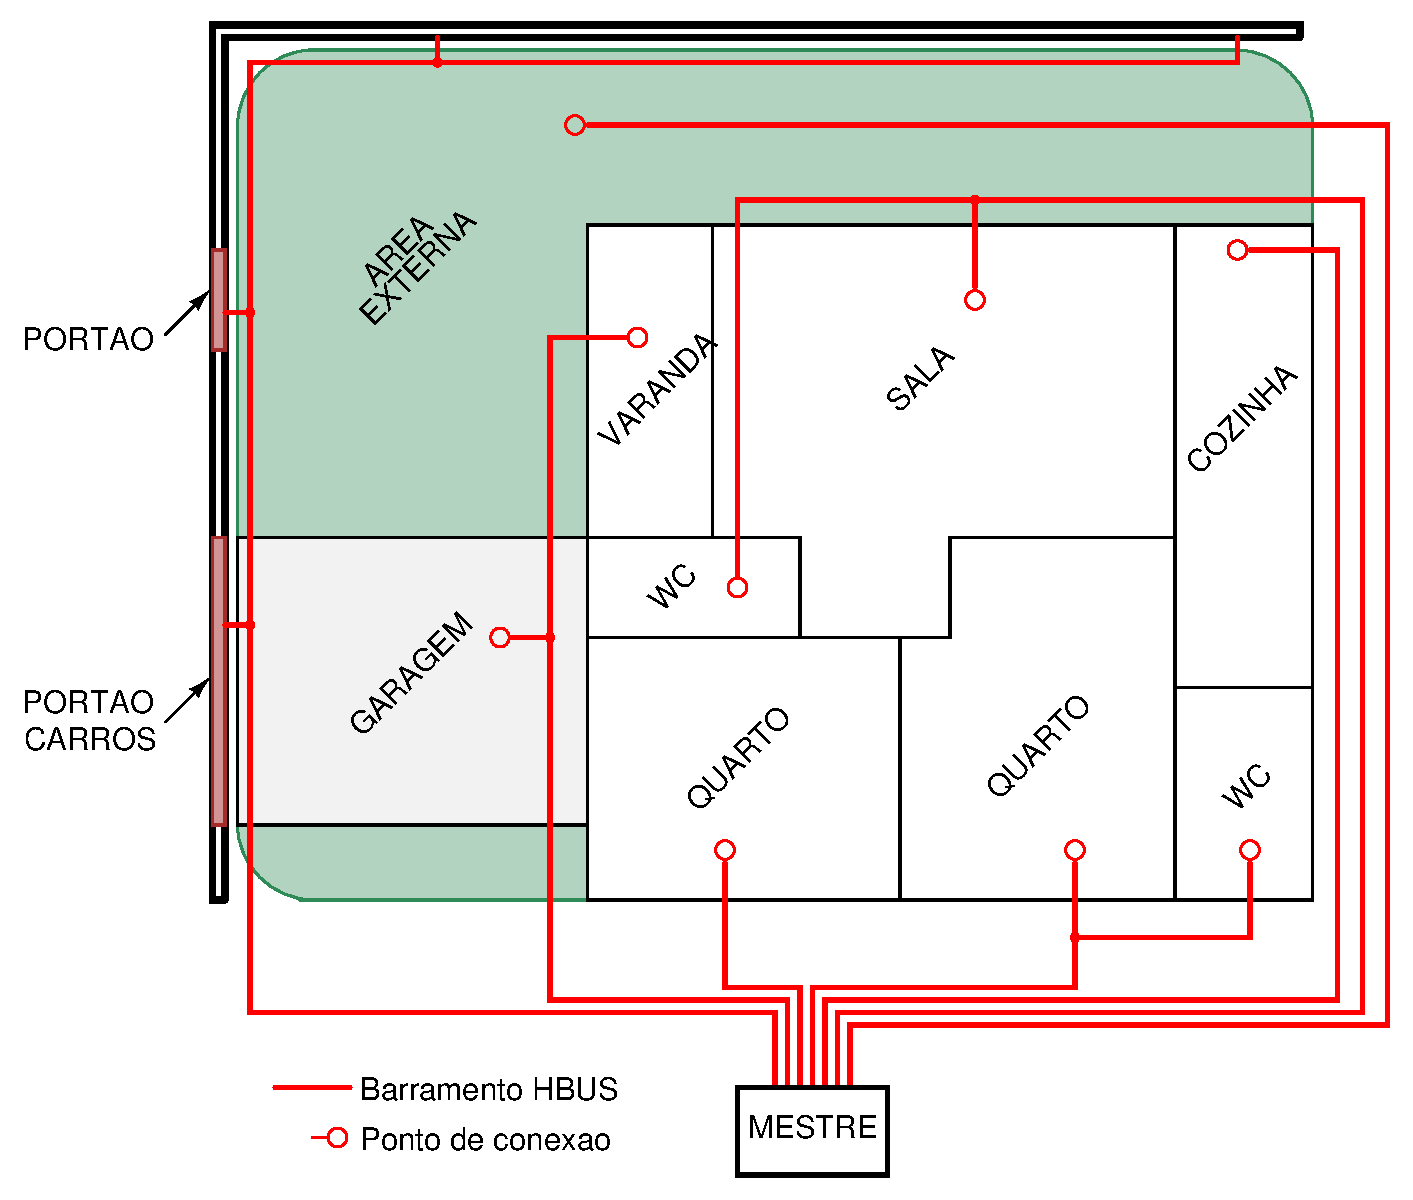
\includegraphics[scale=0.6]{../media/hbus_house.ps}
\caption{Ilustração do uso de barramentos HBUS}
\end{figure}

O barramento HBUS pode ser utilizado para controlar muitas aplicações de uso diário em um ambiente residencial. O esquema mostra o uso de vários barramentos para o controle de uma residência de tamanho médio. No entanto, os barramentos podem ser tanto separados quanto unificados em um só, devido a natureza do sistema que será discutida neste documento.

Na área interna pode ser controlada a iluminação e outros dispositivos quaisquer, podendo incluir interação com o usuário.

Na área externa pode ser controlado o acesso a residência, na forma dos portões para carros e social. Também podem ser instalados diversos tipos de sensores que utilizando o barramento HBUS, disponibilizarão informações ao usuário
